%!TEX root = ../TTK4550-MHT.tex
\section{Linear programming}
\label{sec:ilp}
The aim of this section is to elaborate the use of \gls{lp} to solve the data association problem in \gls{mht} that arises when there are multiple (possible mutual exclusive) possibilities of measurement arrangements within the existing set of tracks. As with any optimization problem, we need an objective function which tells us how good or bad a given assignment is, and a set of constraints that limits the solution to physical limits and our assumptions.

\subsection{Problem formulation}
Multiple optimization formulations of the association problem for multi-target tracking have been proposed through the history. The first was \cite{Morefield1977} where a 0-1 \gls{ilp} was proposed, later an \gls{ilp} scheme with \gls{lp} relaxation and \gls{grp} as solver was proposed by \cite{Storms2003}, and a framework for both association and removal of competing tracks were proposed by \cite{Coraluppi2004}.

All three mentioned publications have essentially the same objective functions, though some use minimize and other use maximize in their formulation. The essence of them all is (\ref{eq:general_objective_funtion}), where $\V{c}$ is a vector of costs (minimize) or scores (maximize) and $\V{\tau}$ is a selection vector, where each row in $\V{c}$ and $\V{\tau}$ represents one branch in the track hypothesis tree.
\begin{equation}
\begin{aligned}
& \underset{\V{\tau}}{\text{min}}
& & \V{c}^T \V{\tau}
\end{aligned}
\label{eq:general_objective_funtion}
\end{equation}

Further, the constraints that shall ensure that each measurement is not assigned to more  than one track are generally formulated as (\ref{eq:general_constraints_equality}) or (\ref{eq:general_constraints_inequality}) , where $\M{A}$ is a binary matrix whose rows are branches in a track hypothesis tree and $\V{b}$ is a vector with ones.
\begin{equation}
\begin{aligned}
&	\M{A} \V{\tau} = \V{b} 	\\
&	\V{\tau} \in \{0,1\}^M
\end{aligned}
\label{eq:general_constraints_equality}
\end{equation}

\begin{equation}
\begin{aligned}
&	\M{A} \V{\tau} \leq \V{b} 	\\
&	\V{\tau} \in \{0,1\}^M
\end{aligned}
\label{eq:general_constraints_inequality}
\end{equation}
The difference between (\ref{eq:general_constraints_equality}) and (\ref{eq:general_constraints_inequality}) originates in some fundamental assumptions in different \gls{mht} versions. When used on a \gls{homht} tree, (\ref{eq:general_constraints_equality}) includes track initialization since it demands that all measurements must be assigned. On the other hand, both (\ref{eq:general_constraints_inequality}) and (\ref{eq:my_constraints}) requires a-priori knowledge about the number of tracks.

In this work, the problem is formulated slightly different, in that there are two sets of constraints (\ref{eq:my_constraints}), one equality and one inequality. The inequality constraints $\M{A_1} \V{\tau} \leq \V{b_1}$ ensures that each measurement are maximum (but not minimum) used one time. The equality constraints $\M{A_2} \V{\tau} = \V{b_2}$ ensures that minimum and maximum one track from each track tree is selected. The complete \gls{ilp} formulation becomes (\ref{eq:my_constraints}), where $\V{\tau}$ is a binary vector with dimension equal the number of leaf nodes in the track forest.
\begin{equation}
\begin{aligned}
&	\underset{\V{\tau}}{\text{max}}
&&	\V{c}^T \V{\tau} \\
&	\text{s.t.}
&&	\M{A_1} \V{\tau} \leq \V{b_1} 	\\
&&&	\M{A_2} \V{\tau} = \V{b_2}	\\
&&&	\V{\tau} \in \{0,1\}^M
\end{aligned}
\label{eq:my_constraints}
\end{equation}
$\M{A_1}$ is a $N_1 \times M$ binary matrix with $N_1$ real measurements and $M$ track hypotheses (all leaf nodes), where $\M{A_1}(l,i)=1$ if hypothesis $l$ are utilizing measurement $i$, $0$ otherwise. The measurements and hypothesis are indexed by the order they are visited by \gls{dfs}. $\M{A_2}$ is an $N_2 \times M$ binary matrix where $N_2$ is the number of targets in the cluster and $\M{A_2}(l,j)=1$ if hypothesis $l$ belongs to target $j$. $\V{b_1}$ is a $N_1$ long vector with ones and $\V{b_2}$ is a $N_2$ long vector with ones. $\V{c}$ is a $M$ long vector with a measure of the goodness of the track hypotheses. For example, in Figure \ref{fig:hyp-tree} at time step 2, the $\M{A}$ matrices and $\V{C}$ vector would be (\ref{eq:example_matrices}).
\begin{figure}[H]
\centering
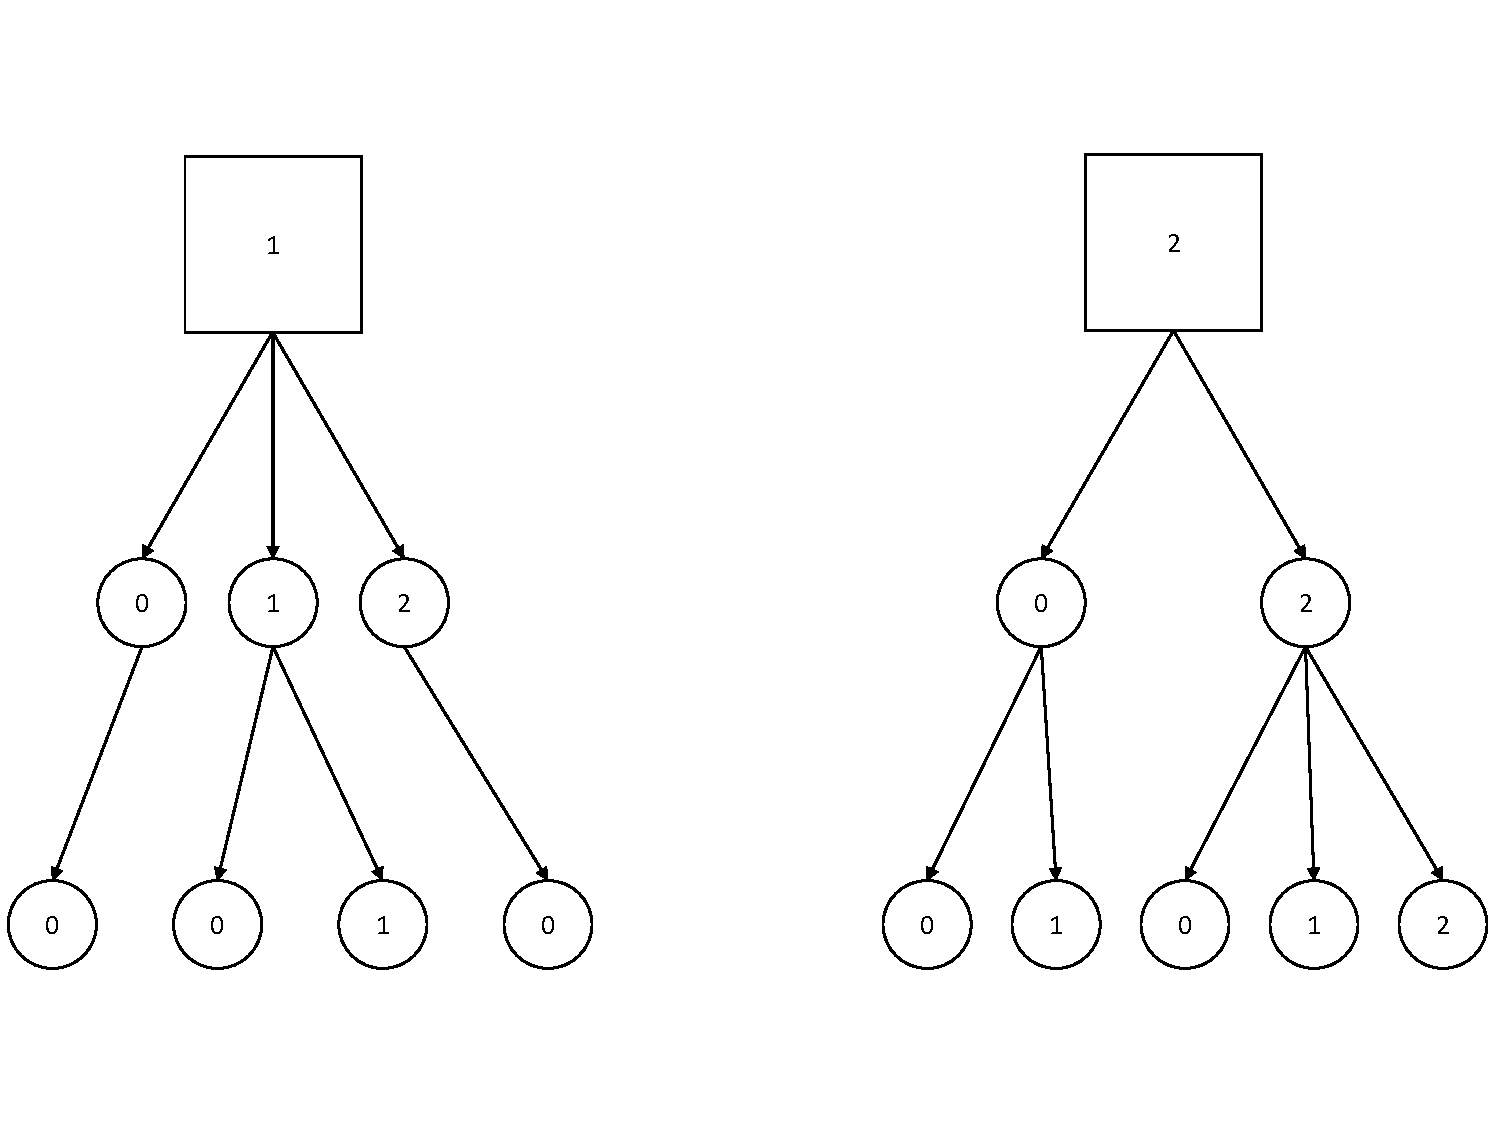
\includegraphics[clip, trim=0cm 2.5cm 0cm 2.5cm, width = .7\textwidth]{Track-tree}
\caption{Track hypothesis tree}
\label{fig:hyp-tree}
\end{figure}

\begin{equation}
\begin{split}
\M{A_1} &=\begin{bmatrix}
		0 & 1 & 1 & 0 & 0 & 0 & 0 & 0 & 0 \\
       	0 & 0 & 1 & 0 & 0 & 1 & 0 & 1 & 0 \\
       	0 & 0 & 0 & 1 & 0 & 0 & 1 & 1 & 1 \\
       	0 & 0 & 0 & 0 & 0 & 0 & 0 & 0 & 1 \\
     	\end{bmatrix}
\V{b_1} = 	\begin{bmatrix}
			1 \\ 1  \\ 1 \\ 1
			\end{bmatrix} \\
\M{A_2} &=\begin{bmatrix}
		1 & 1 & 1 & 1 & 0 & 0 & 0 & 0 & 0 \\
       	0 & 0 & 0 & 0 & 1 & 1 & 1 & 1 & 1 \\
     	\end{bmatrix} 
\V{b_2} = 	\begin{bmatrix}
			1 \\ 1
			\end{bmatrix} \\
\V{c} &=\begin{bmatrix}
		\lambda_1 & \lambda_2 & \lambda_3 & \lambda_4 & \lambda_5 & \lambda_6 & \lambda_7 & \lambda_8 & \lambda_9
		\end{bmatrix}^T \\
\end{split}
\label{eq:example_matrices}
\end{equation}

The explicit enumeration that becomes necessary when creating these $\M{A}$ matrices is exhaustive since dimension of $\V{\tau}$, which is equal to the number of leaf nodes in the track forest, can be very large. Both $\M{A}_1$ and $\M{A}_2$ grows quadratically with the number of track hypotheses and real measurements or number of targets respectively.
% $N_1$ is proportional with the number of targets and history steps (N-scan). 

\subsection{Solvers}
There are a lot of of-the-shelf \gls{ilp} and \gls{milp} solvers on the marked, both free open source and commercial. Since our problem is formulated on standard form, it can easily be executed on several solvers, and we can compare runtime and performance. In this report, the following solvers are tested:
\begin{itemize}
\item CBC 		(Free, COIN-OR)
\item CPLEX 	(Commercial (Free academic),  IBM)
\item GLPK 		(Free, GNU)
\item Gurobi 	(Commercial (Free academic), Gurobi)
\end{itemize}